\section{Desarrollo Realizado}

\subsection{Arquitectura de la Solución}
    \begin{frame}[c,shrink]{Arquitectura de la Solución}
    \begin{figure}
        \centering
        
\includegraphics[width=0.8\textwidth]{images/diagrama-arquitectura.png}
    \end{figure}
    \end{frame}


\subsection{Tecnologías}
    \begin{frame}[c,shrink]{Tecnologías empleadas}
        \begin{block}{Heredadas del TFG}
            \begin{itemize}
                \item Java / Spring Boot, Spring Data, JPA / Hibernate.
                \item React + Redux + RTK Query + Material UI.
                \item MapLibre + MapTiler.
                \item PostgreSQL + PostGIS.
                \item Open Weather Map.
            \end{itemize}
        \end{block}
        \begin{block}{Nuevas incorporaciones}
            \begin{itemize}
                \item OpenAPI / API-first (generación automática de DTOs y controladores).
                \item Kotlin + Jetpack Compose para Android.
                \item Firebase Cloud Messaging (notificaciones push).
                \item Testcontainers.
                \item Motor de reglas en JSONB.
            \end{itemize}
        \end{block}
    \end{frame}

\subsection{Diagramas C4}
    \begin{frame}[c]{C4 - Diagrama de contexto}
        \begin{figure}
            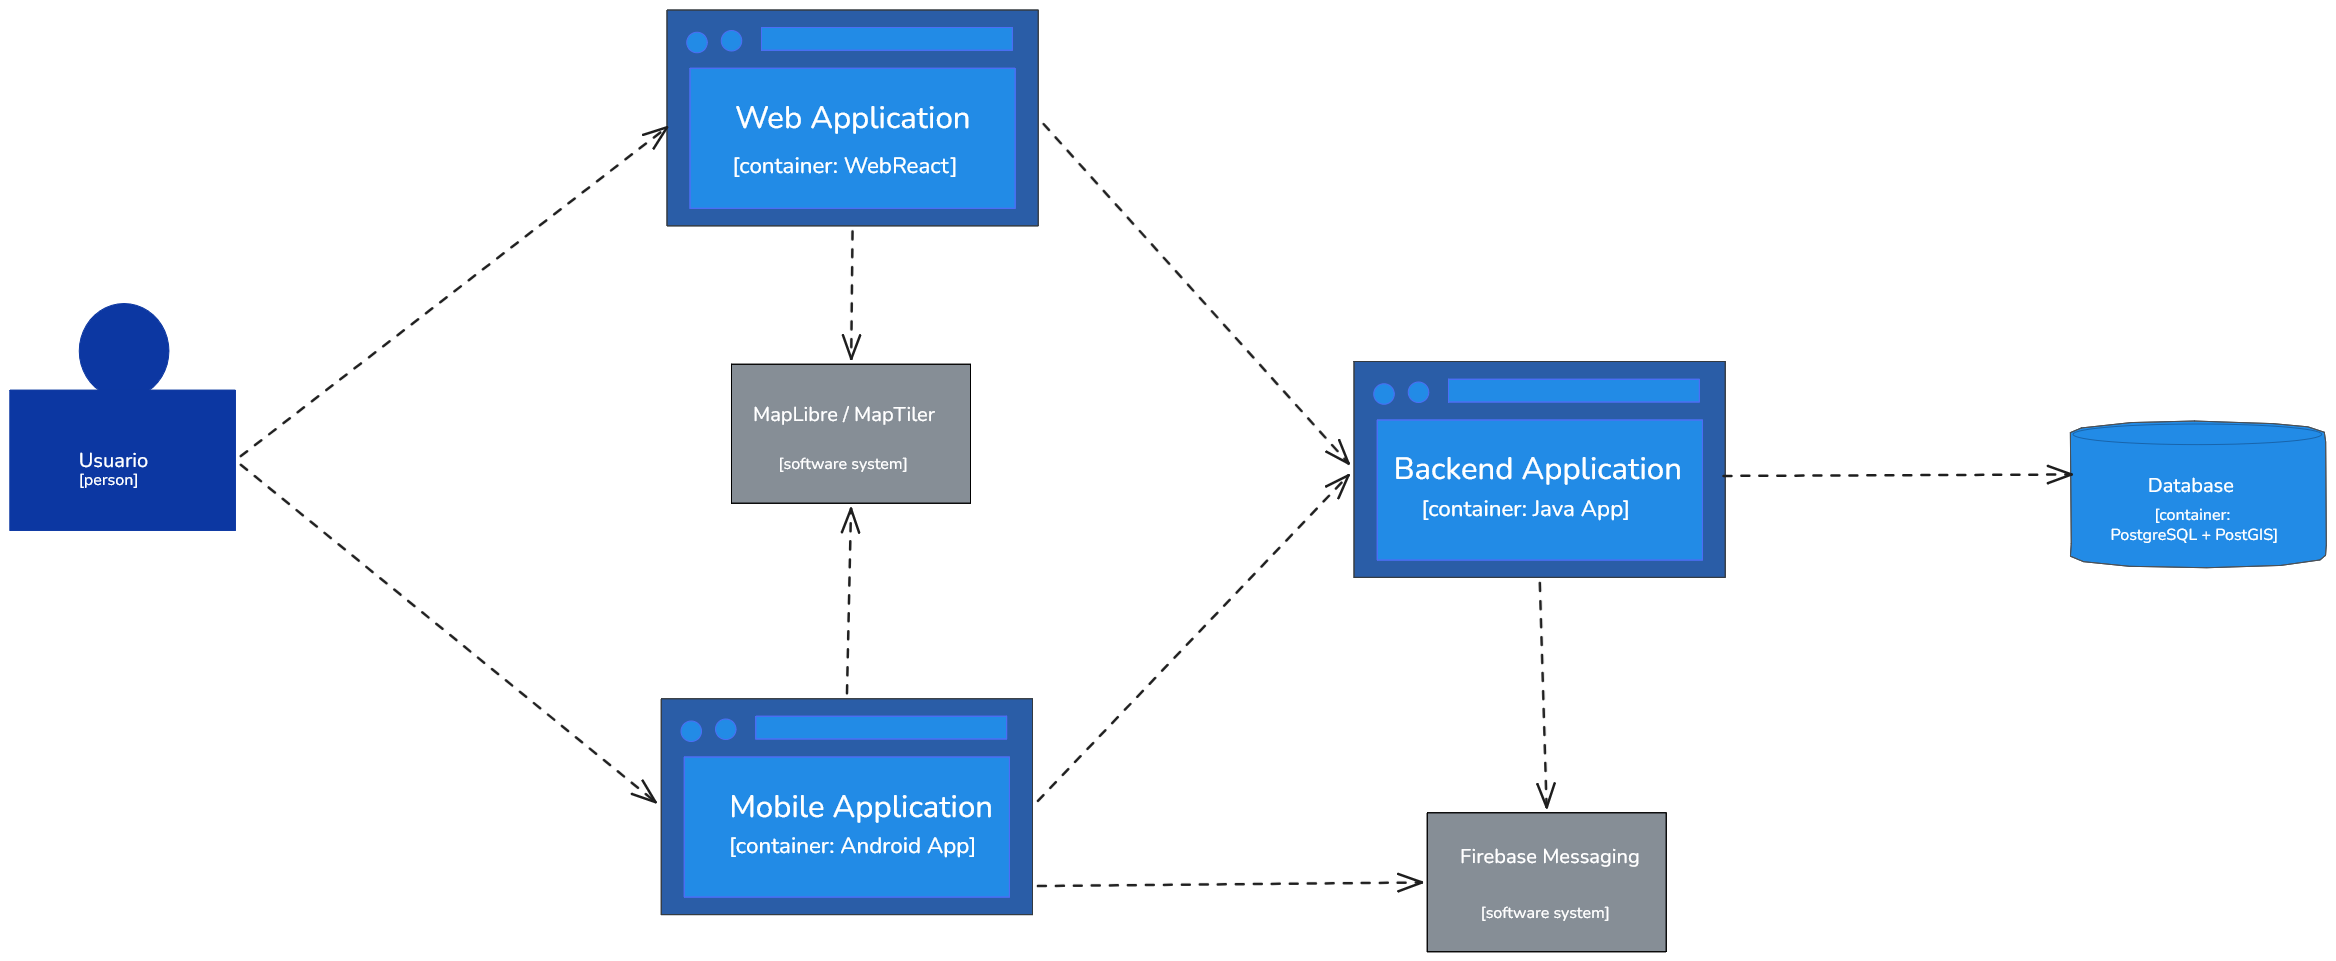
\includegraphics[width=0.9\textwidth]{images/c4_contextual.png}
        \end{figure}
    \end{frame}



\subsection{Planificación y Metodología}
    \begin{frame}[c,shrink]{Planificación y Metodología}
        \begin{block}{Metodología}
            \begin{itemize}
                \item Enfoque iterativo e incremental (9 sprints de 2 semanas).
                \item Reuniones de revisión mensuales con el tutor.
                \item Cada sprint: análisis, diseño, implementación y pruebas.
            \end{itemize}
        \end{block}
        \begin{block}{Datos de esfuerzo}
            \begin{itemize}
                \item \textbf{Estimado:} 405 horas.
                \item \textbf{Real:} 428 horas (desviación del 5,7\%).
                \item \textbf{Coste real:} 6.417,18~\euro.
            \end{itemize}
        \end{block}
    \end{frame}

\subsection{Análisis de requisitos}
    \begin{frame}[c,shrink]{Actores del sistema}
        \begin{block}{Jerarquía acumulativa de permisos}
            \begin{itemize}
                \item \textbf{Usuario no autenticado:} mapa general y creación de avisos.
                \item \textbf{Usuario autenticado:} consulta de avisos propios y notificaciones.
                \item \textbf{Miembro de equipo:} información operativa de su equipo y asignaciones.
                \item \textbf{Responsable de equipo:} gestión de equipos y vehículos.
                \item \textbf{Coordinador:} gestión completa de usuarios, organizaciones, emergencias, asignaciones y reglas.
            \end{itemize}
        \end{block}
    \end{frame}

\subsection{Diseño}
    \begin{frame}[c,shrink]{Backend - Modelo de dominio(1/2)}
        \begin{figure}
            \centering
            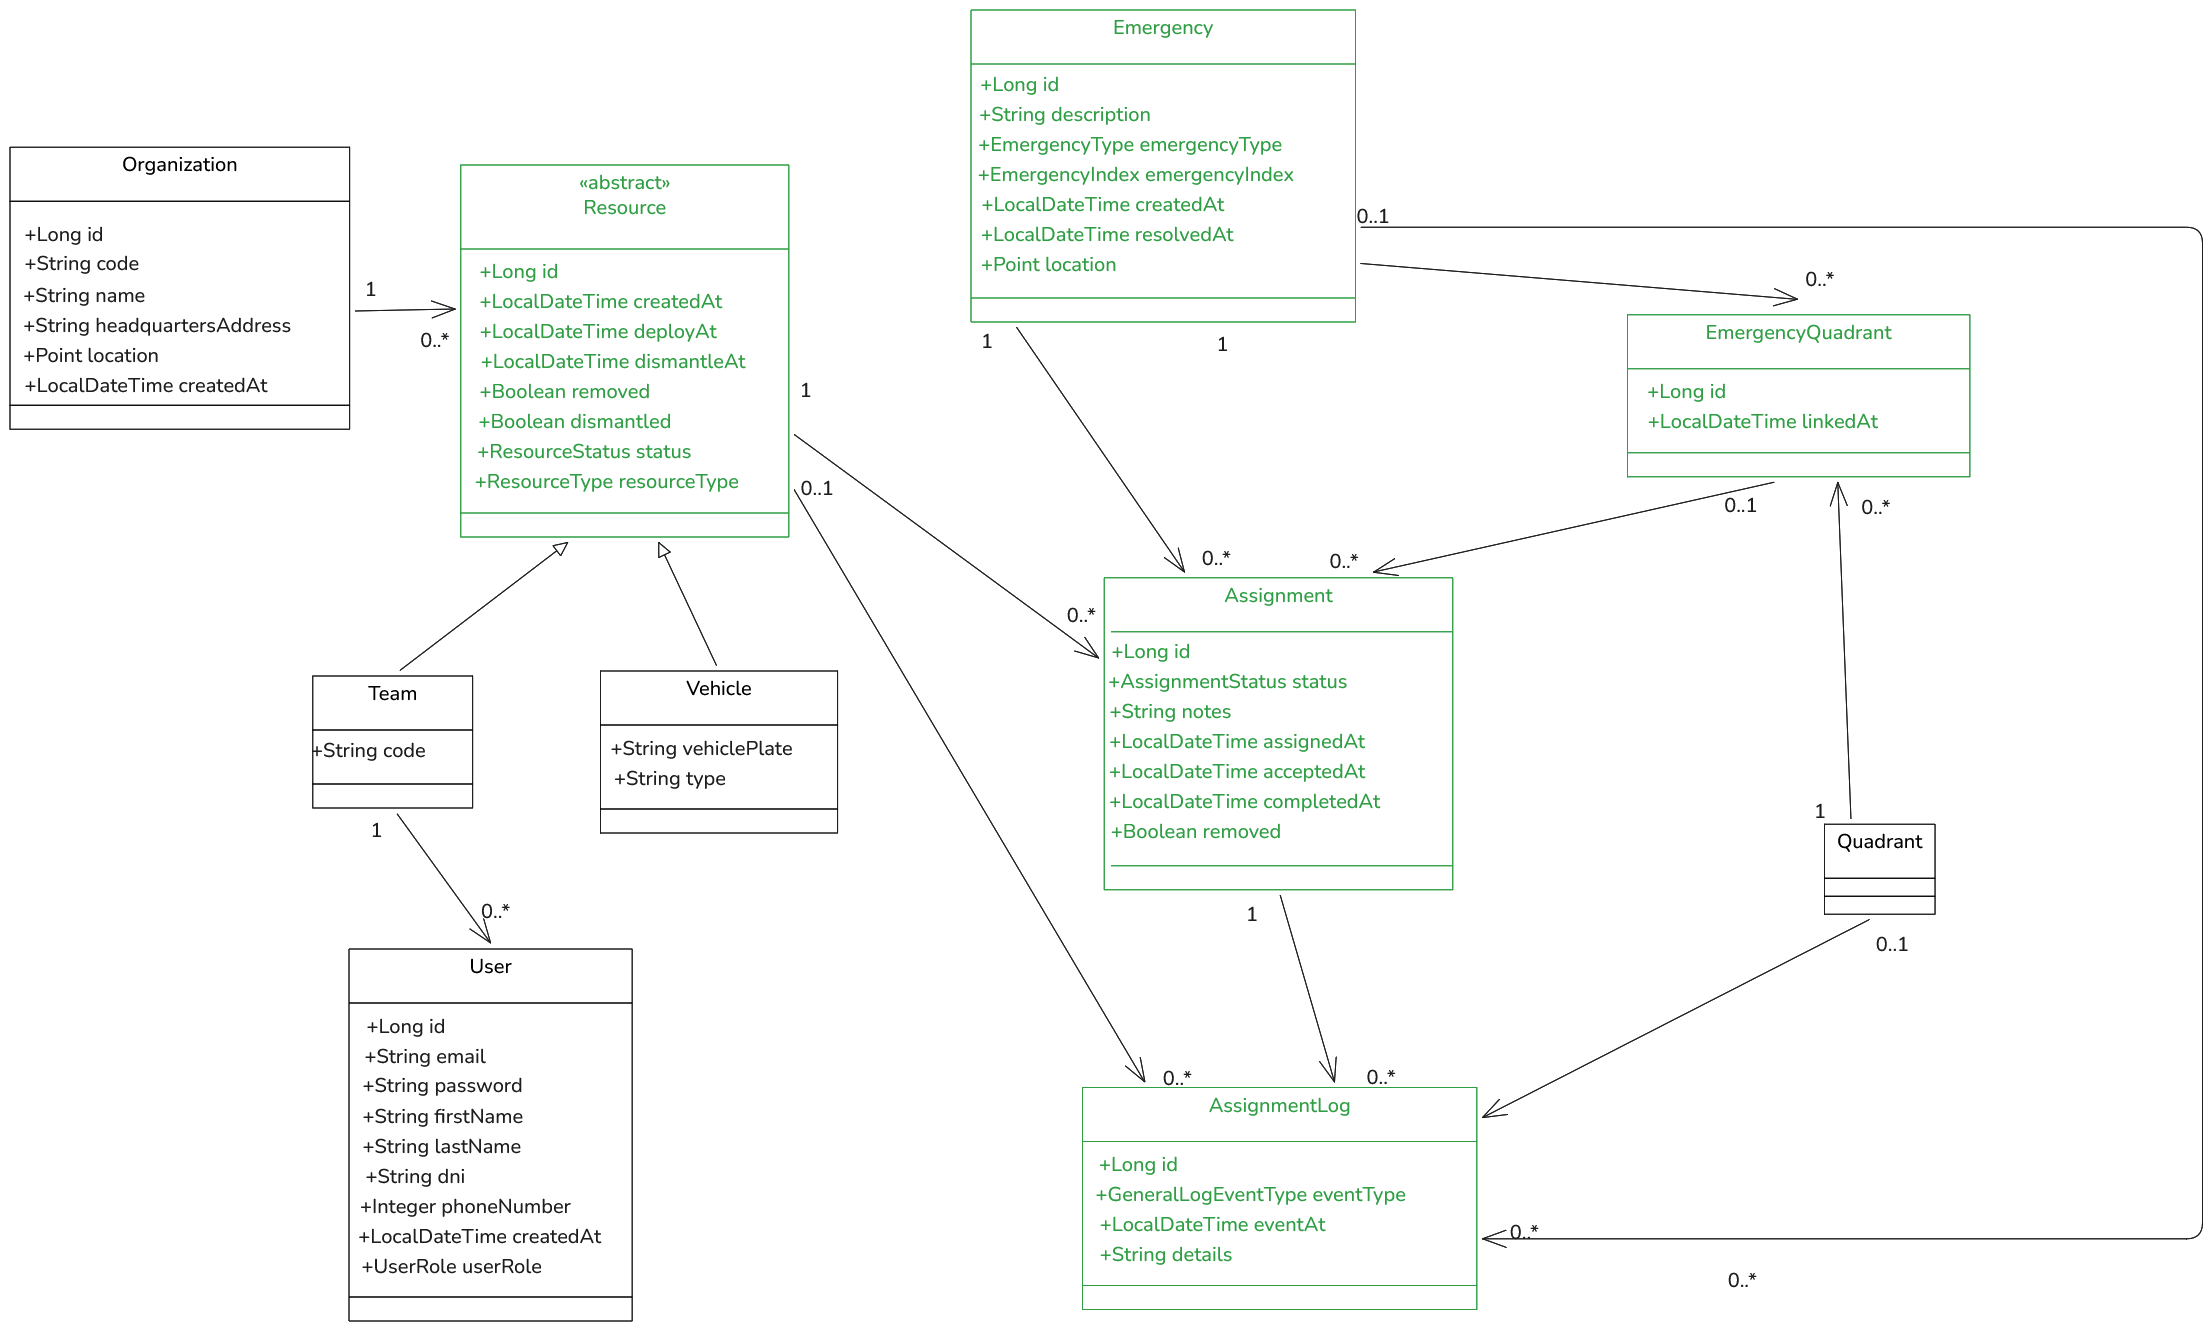
\includegraphics[width=0.95\textwidth]{images/modelo_dominio_central.png}
        \end{figure}
        
    \end{frame}

    \begin{frame}[c,shrink]{Backend - Modelo de dominio(2/2)}
        \begin{figure}
            \centering
            \begin{minipage}{0.30\textwidth}
                \centering
                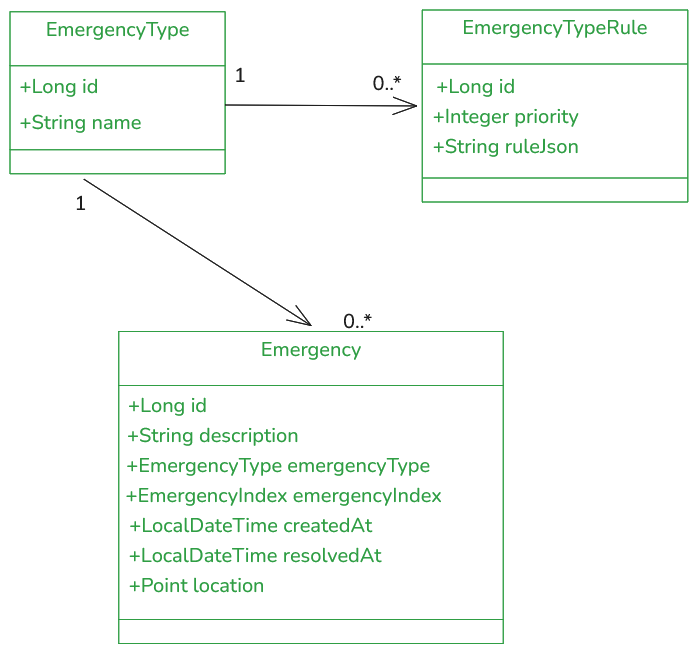
\includegraphics[width=0.9\textwidth]{images/modelo_dominio_emergencias.png}
            \end{minipage}
            \hfill
            \begin{minipage}{0.69\textwidth}
                \centering
                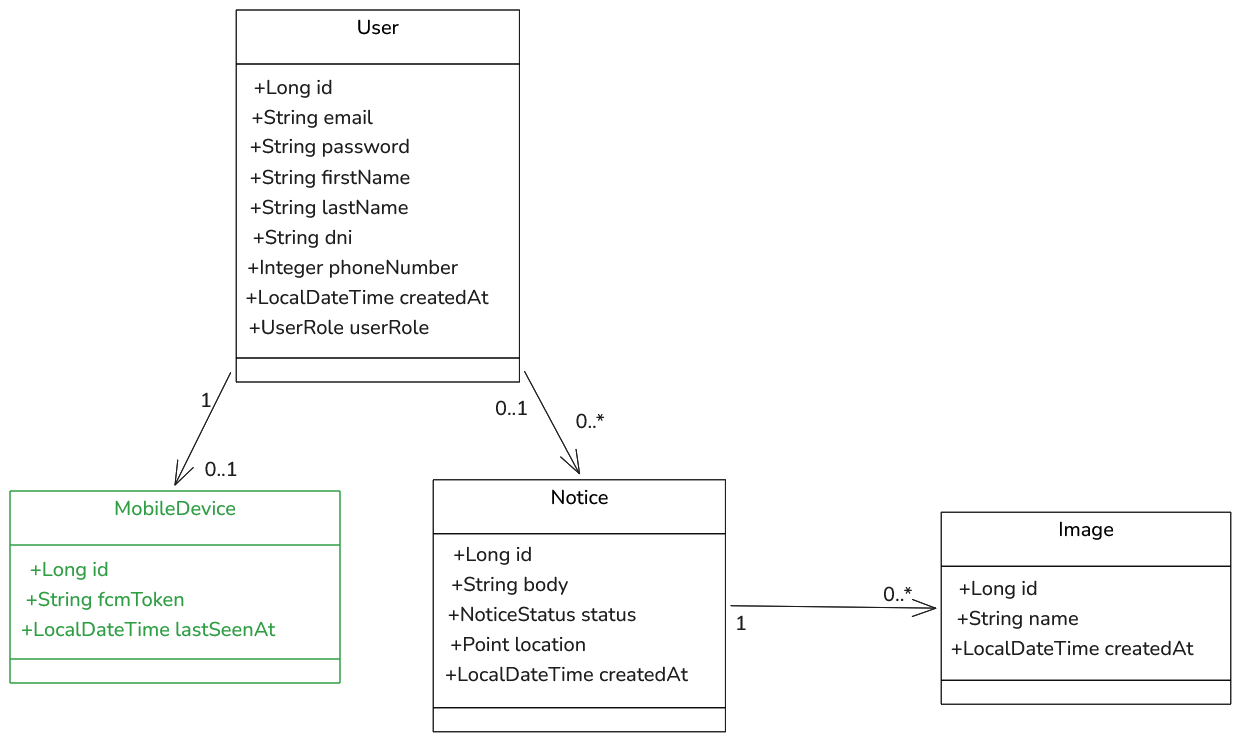
\includegraphics[width=0.9\textwidth]{images/modelo_dominio_usuarios.png}
            \end{minipage}
        \end{figure}
    \end{frame}

    \begin{frame}[c,shrink]{Backend - Lógica de negocio}  
        \begin{figure}
            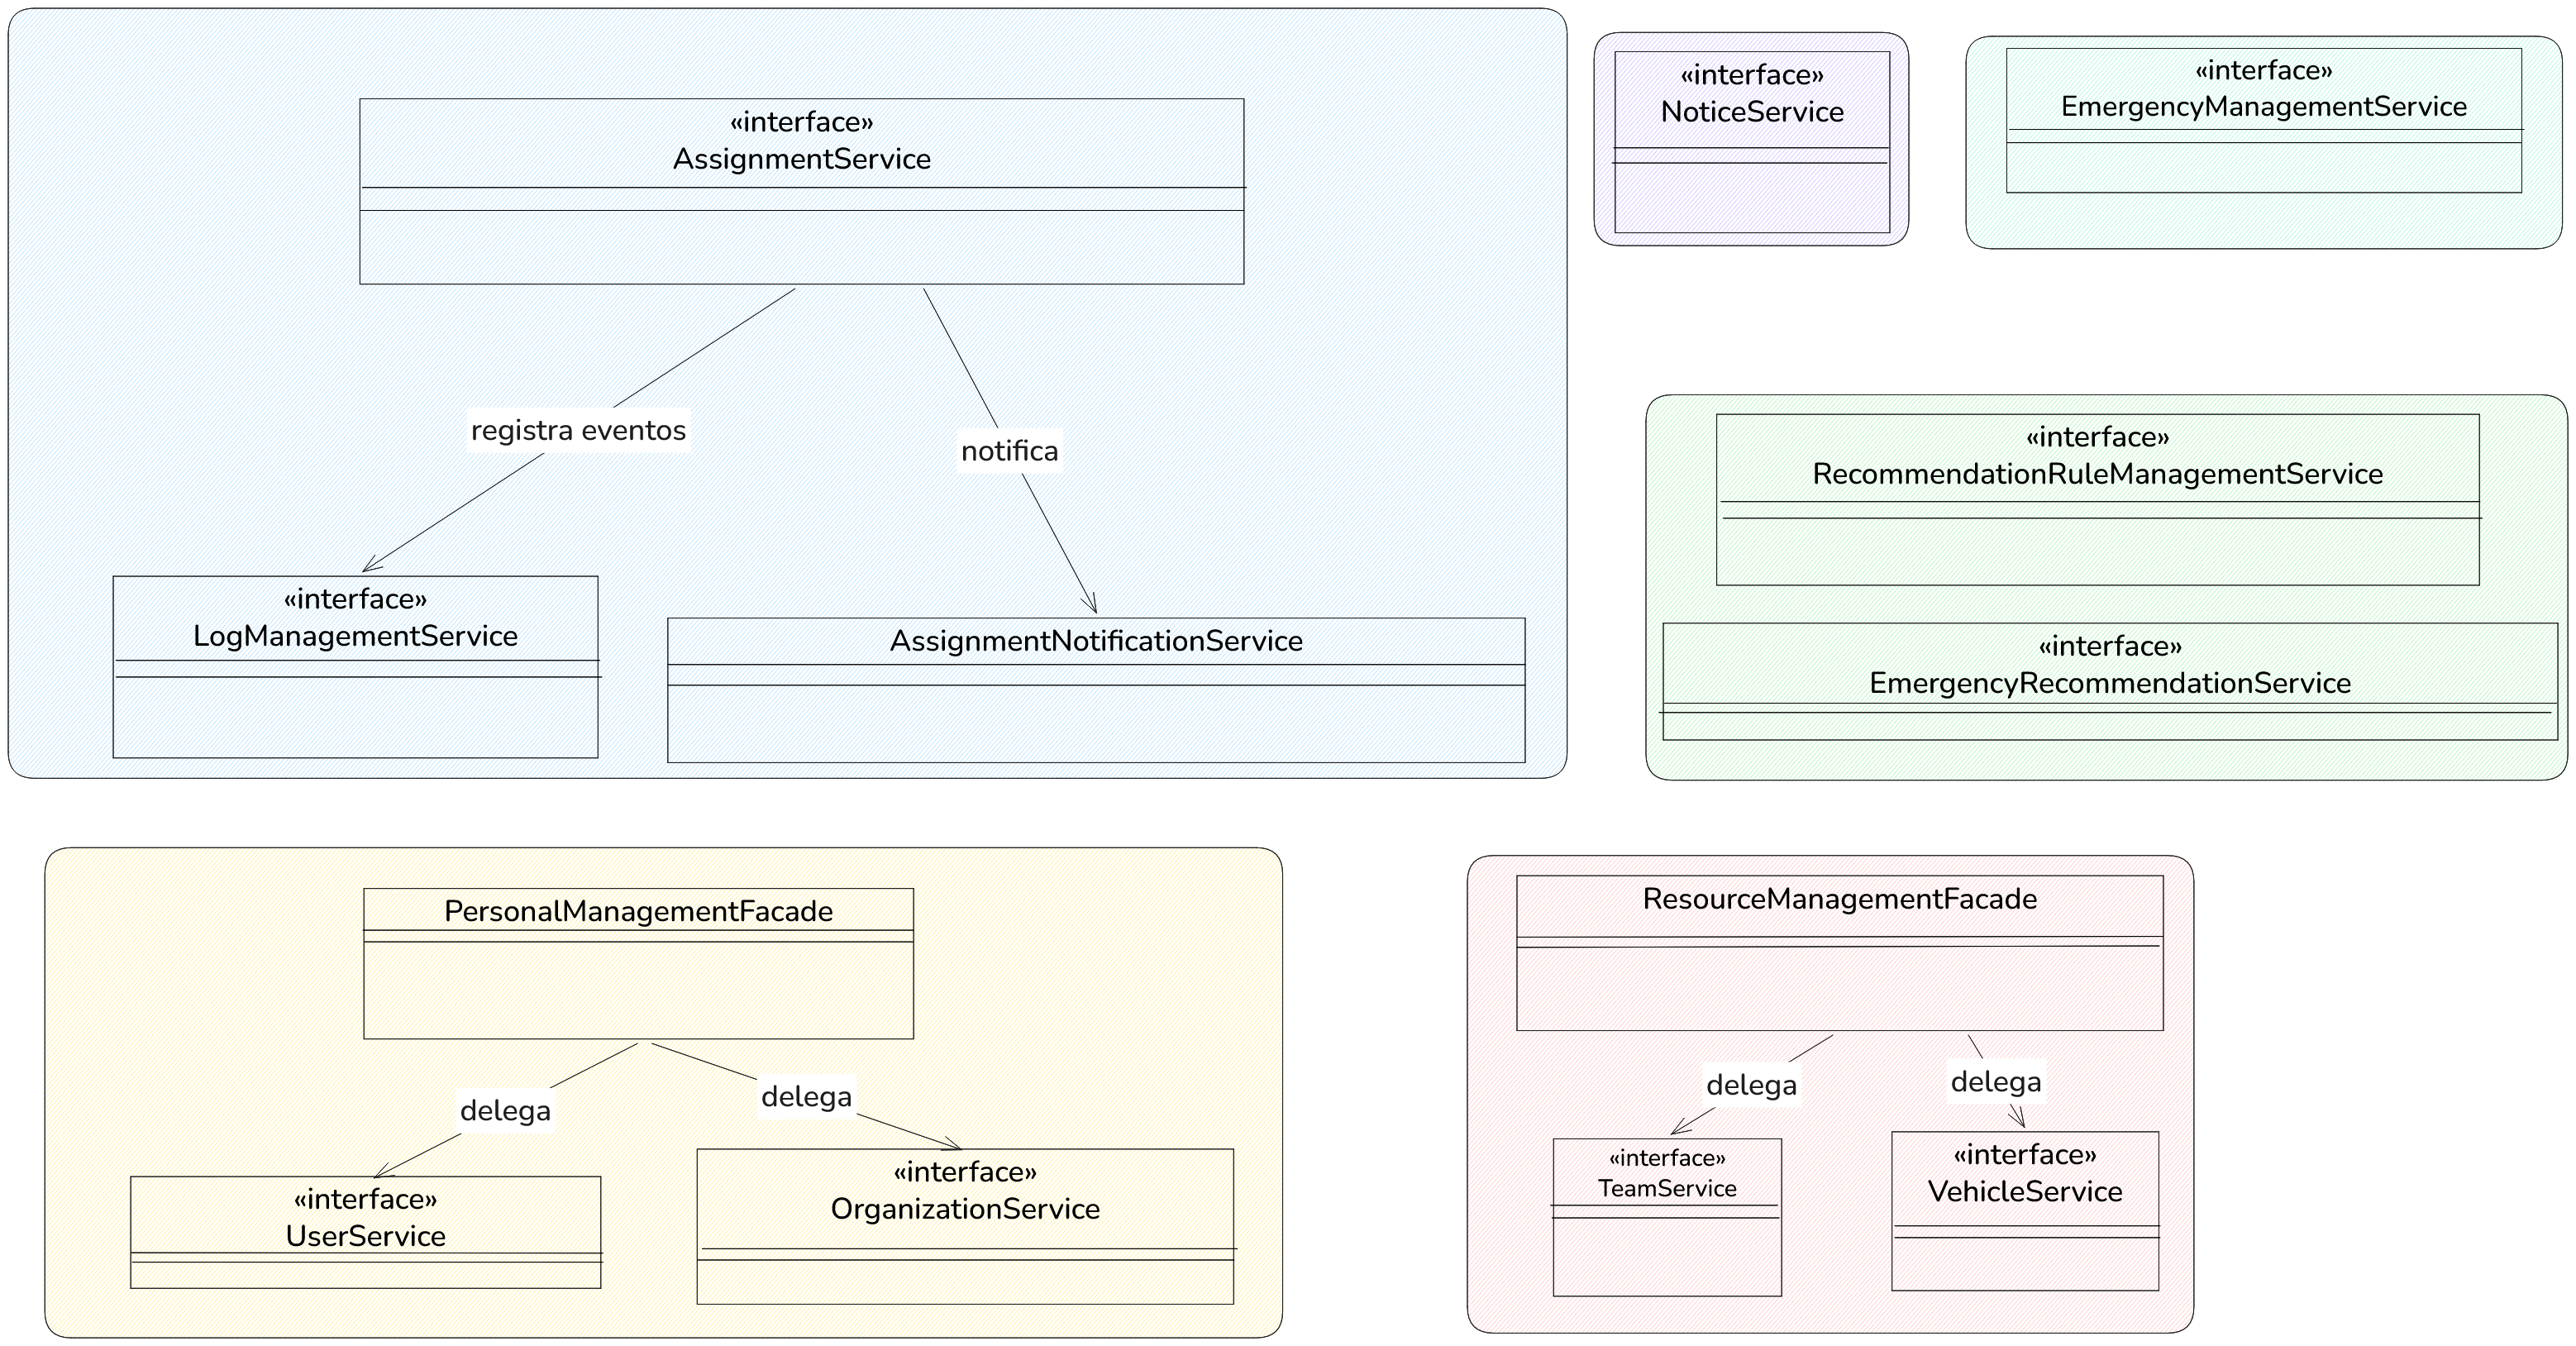
\includegraphics[width=0.90\textwidth]{images/diagrama-negocio.png}
        \end{figure}
    \end{frame}


    \begin{frame}[c]{Backend - DAOs y Repositorios}
        \begin{figure}
            \centering
            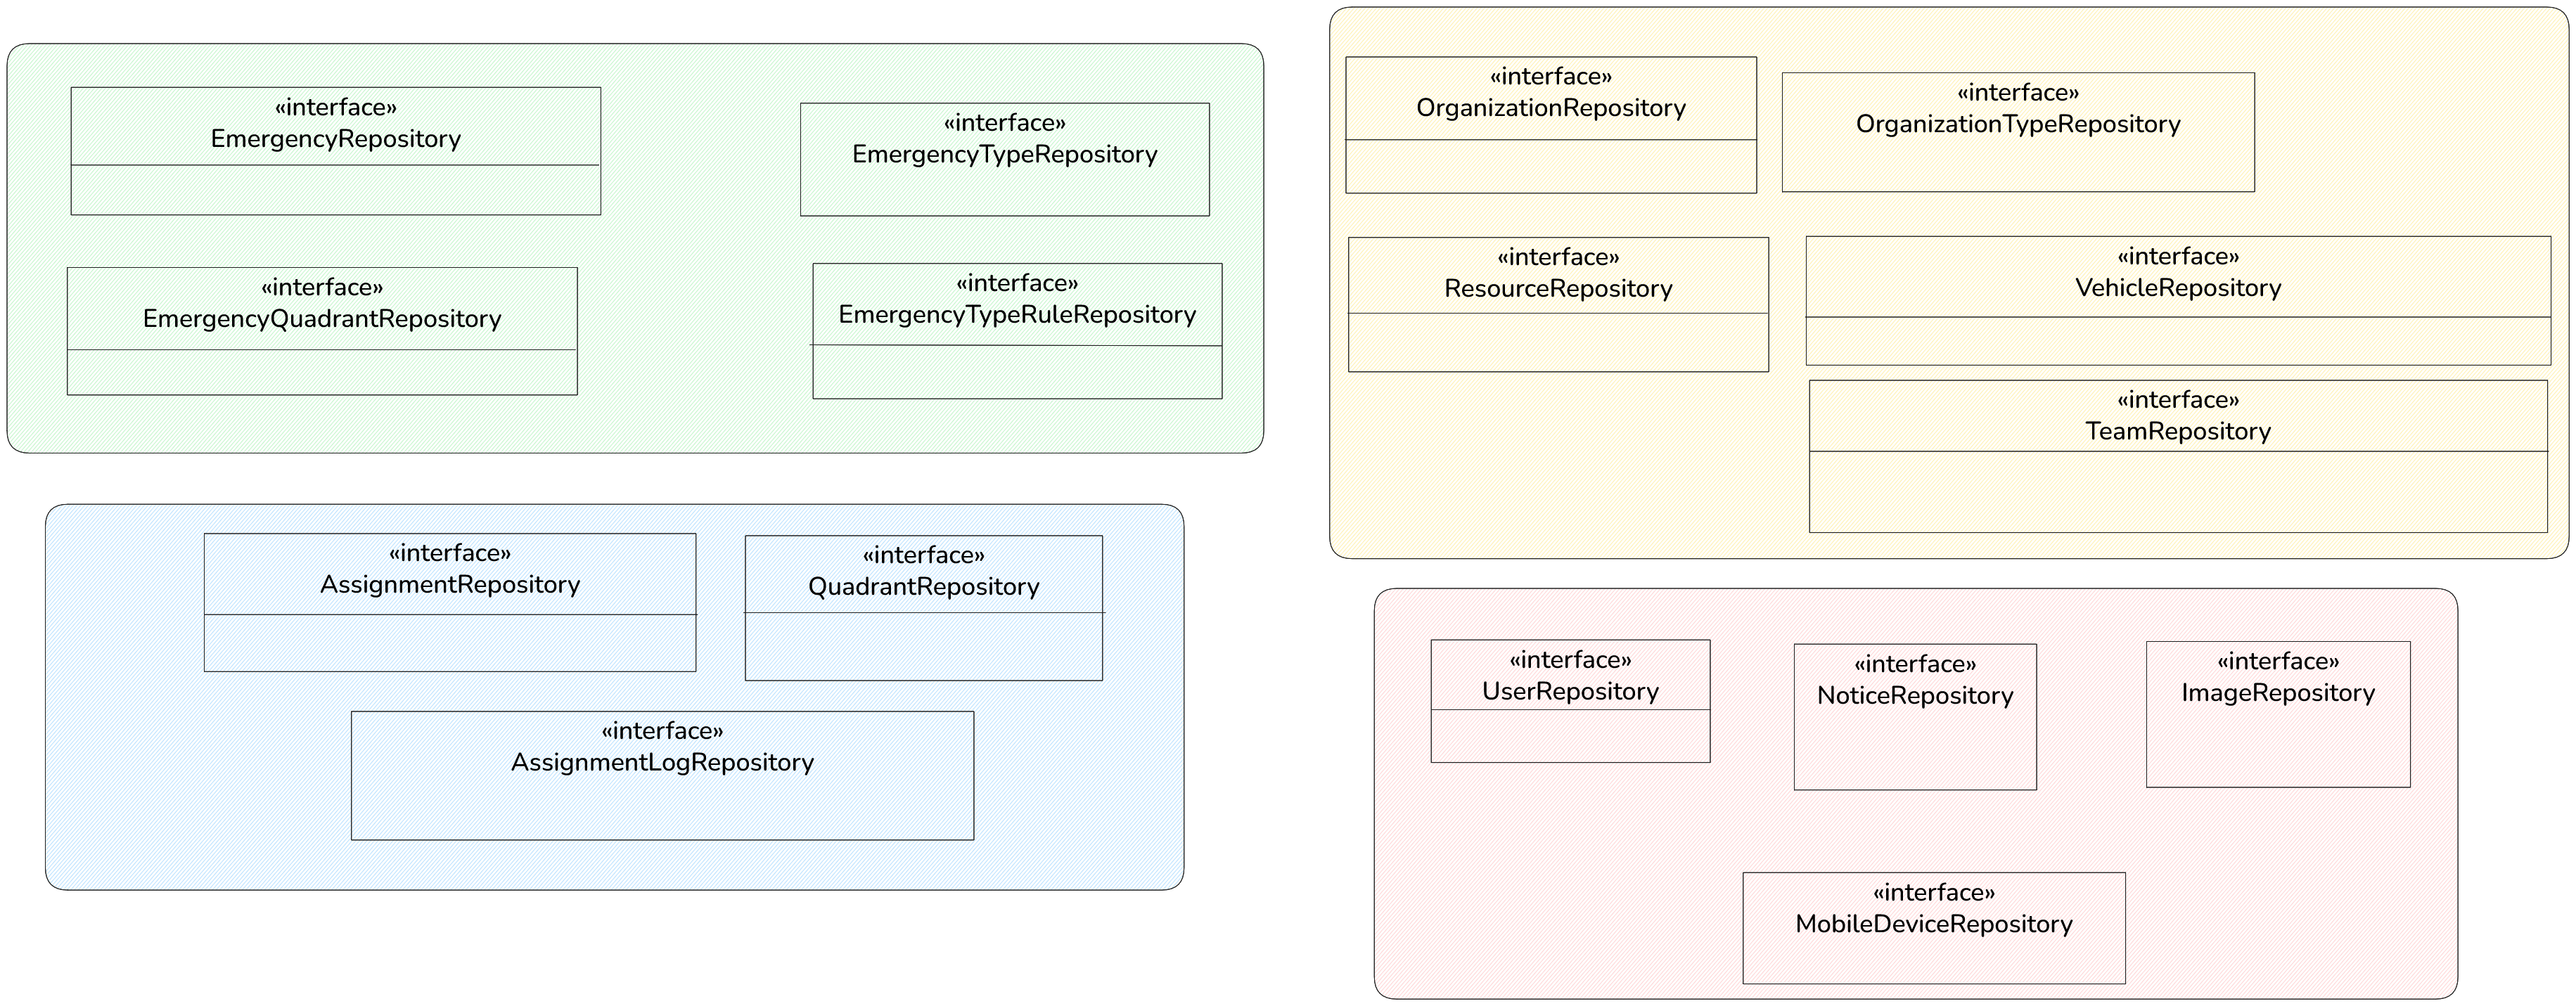
\includegraphics[width=0.93\textwidth]{images/diagrama-repositorios.png}
        \end{figure}
    \end{frame}

    \begin{frame}[c]{Backend - Controladores REST}
        \begin{figure}
            
\includegraphics[width=0.65\textwidth]{images/swagger.png}
            \caption{Imagen resumen de los Endpoints implementados.}
        \end{figure}
    \end{frame}

    \begin{frame}[c]{Frontend - Diagrama de contenedores}
        \begin{figure}
            
\includegraphics[width=0.85\textwidth]{images/c4_container_frontend.png}
        \end{figure}
    \end{frame}

   \begin{frame}[c]{Android - Diagrama de contenedores}
        \begin{figure}
            
\includegraphics[width=0.7\textwidth]{images/c4_container_android.png}
        \end{figure}
    \end{frame}

   \begin{frame}[c]{Android - Diagrama secuencia Notificación push}
        \begin{figure}
            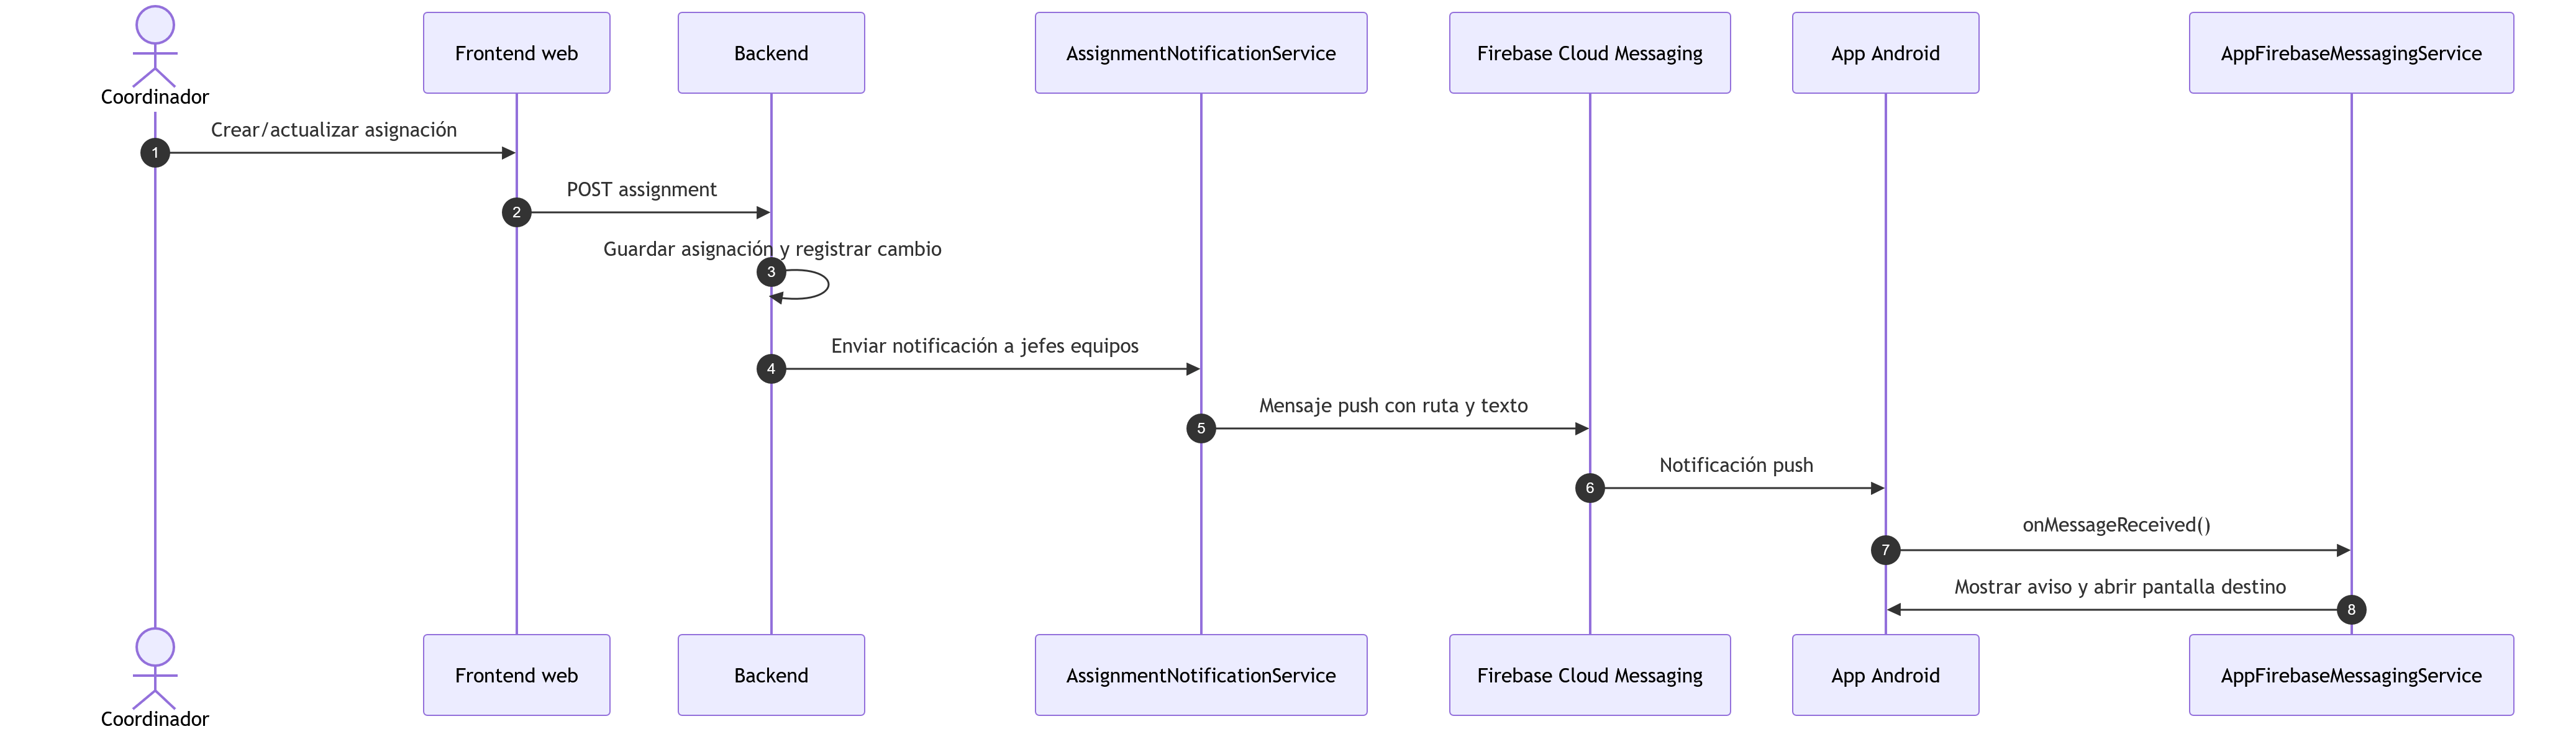
\includegraphics[width=\textwidth]{images/diagrama-secuencia-fcm.png}
        \end{figure}
    \end{frame}

    \begin{frame}[c]{Internacionalización y localización}
        Los tres módulos soportan \textbf{español}, \textbf{inglés} y \textbf{gallego}:
        \begin{itemize}
            \item \textbf{Backend:} Ficheros \texttt{messages.properties} con \texttt{MessageSource} de Spring.
            \item \textbf{Frontend:} Librería \texttt{i18next} con detección automática de idioma.
            \item \textbf{Android:} \texttt{LocaleHelper} con persistencia en preferencias.
        \end{itemize}
    \end{frame}

   

\subsection{Pruebas}
    \begin{frame}[c,shrink]{Estrategia de pruebas}

        \begin{block}{Backend}
            \begin{itemize}
                \item Unitarias: JUnit 5 + Mockito 
                \item Integración: Testcontainers con PostgreSQL/PostGIS.
                \item Cobertura elevada en capa de servicios.
            \end{itemize}
        \end{block}
        
        \begin{block}{Frontend}
            \begin{itemize}
                \item Vitest + React Testing Library.
                \item Lógica pura: validaciones, transformación de coordenadas.
                \item Componentes clave: renderizado y comportamiento.
            \end{itemize}
        \end{block}
        
        \begin{block}{Android}
            \begin{itemize}
                \item Unitarias locales: utilidades, coordenadas, fechas.
                \item Instrumentadas: verificación de Activities e Intents.
            \end{itemize}
        \end{block}
    \end{frame}
